\documentclass[14]{article}

% Used packages
\usepackage{apacite}
\usepackage[12pt]{moresize}
%\usepackage[numbers,sort&compress]{natbib}
\usepackage{blindtext}
\usepackage{enumitem}
\usepackage{xcolor}
\usepackage[explicit,noindentafter]{titlesec}
\usepackage[rightcaption]{sidecap}
\usepackage{caption}
\usepackage{float}
\usepackage{csquotes}
\usepackage{titling}
\usepackage{titlesec}
\usepackage{graphicx} %package to manage images
\graphicspath{{images/}}



\titlespacing\section{1pt}{12pt plus 0pt minus 0pt}{6pt plus 0pt minus 0pt}
\titlespacing\subsection{1pt}{12pt plus 4pt minus 2pt}{6pt plus 2pt minus 2pt}
\titlespacing\subsubsection{1pt}{12pt plus 4pt minus 2pt}{6pt plus 2pt minus 2pt}
\titlespacing\paragraph{1pt}{12pt plus 4pt minus 2pt}{6pt plus 2pt minus 2pt}

% New commands
\newcommand{\addsection}[3]{\addtocontents{toc}{\protect\contentsline{section}{\protect\numberline{#1}#2}{#3}}}
\newcommand{\addsubsection}[3]{\addtocontents{toc}{\protect\contentsline{subsection}{\protect\numberline{#1}#2}{#3}}}
\newcommand{\itab}[1]{\hspace{0em}\rlap{#1}}
\newcommand{\tab}[1]{\hspace{.5\textwidth}\rlap{#1}}
\newcommand{\Csh}{C{\lserif\#}}


\begin{document}
\author{\textbf{Faculty of Sciences and Bio-Engineering Sciences}\\[2\baselineskip]\newline\textbf{Arthur Chomé - 0529279}}

\date{ \LARGE Assignment 2: Statistics}
\title{\vspace{-8cm}}%\underline{Everything is connected}}

\maketitle

\section{Introduction}
As a second assignment for the course Methods for Scientific Research, we have to fulfil four statistical exercises. Further details of which can be found in the assignment document available on Canvas. Also provided were the datasets to be used for the exercises, based on our student number (0529279) the set number calculator\footnote{\protect\url{https://ai.vub.ac.be/~bart/statsnumbers.html}} assigned us with the sets 4, 1, 4, 3 for the four respective questions. All tests, charts and diagrams were generated using IBM's SPSS Statistics package version 23\footnote{\protect\url{https://en.wikipedia.org/wiki/SPSS}} released in 2015. 

\section{Question 1}
The used dataset --set 4 for the first question-- was gathered by way of an experiment measuring the resonance frequencies of two types of crystal oscillators (variables x1 and x2) needed to provide timing information for high performance hardware. 

\subsection{Diagram}
The use of boxplots is a standardized way of displaying the distribution of data based on the five number summary: minimum, first quartile, median, third quartile, and maximum. Between the first and third quartile lies 50 percent of all data with the median being the middle value of the whole set. Between the maximum and minimum lies about 99.75 percent of all data.

\begin{figure}[!htb]
	\includegraphics[width=1.0\textwidth]{img/question1/Question1_Boxplot.PNG}
	\captionsetup{width=1.0\textwidth}
	\centering
	%\caption{Given boxplots show that both variables have an evenly distributed range. Dataset x1 however has a wider distribution of its data with the maximum and minimum of the data being further away from the median than in dataset x2. } 
\end{figure}
\mbox{}\\ 

\paragraph{Explanation}\mbox{}\newline
Datasets that have a normal distribution have symmetrical boxplots with the means being in the center. This is clearly the case for both datasets. Set x1 however has a wider distribution of its data with the maximum and minimum of the data being further away from the median than in dataset x2. 
\newline
The use of boxplots is a standardized way of displaying the distribution of data based on the five number summary: minimum, first quartile, median, third quartile, and maximum. Using boxplots gives us a simple way of detecting symmetry and distribution of datasets and comparing them between each other. 

\subsection{Welch's T-test}
Based on the experiment's description, we want to see if the same variable applied on two different populations (e.g. different groups of oscillator crystals) makes for a difference of the means of variables. Because the variance of both datasets differs significantly, a normal T-test would not be reliable in doing so. 
\newline
This is why we settle for Welch's T-test because it is robust even when the sample size or the variance is unequal. In this case, an independent T-test is the best option. Our null hypothesis in this case is that the means of both data collections do not differ. 

\begin{figure}[!htb]
	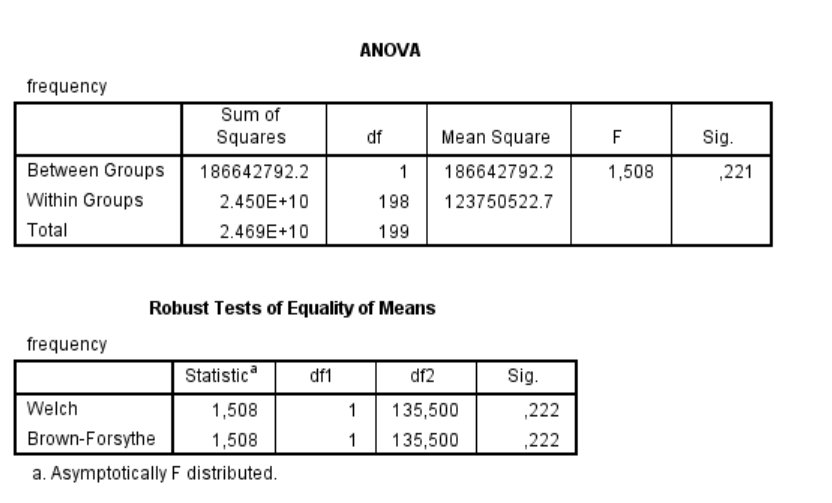
\includegraphics[width=1.0\textwidth]{img/question1/question1_b.PNG}
	\captionsetup{width=1.0\textwidth}
	\centering
	%\caption{Given boxplots show that both variables have an evenly distributed range. Dataset x1 however has a wider distribution of its data with the maximum and minimum of the data being further away from the median than in dataset x2. } 
\end{figure}

\paragraph{Null \& Alternative Hypothesis}\mbox{}\\
For this T-test, our null hypothesis is that no significant difference in means exists between the datasets x1 and x2 of the oscillator crystals. The alternative would be that a significant difference in means exists between the two. All hypothesis tests make use of a p-value\footnote{\protect\url{https://en.wikipedia.org/wiki/P-value}} to weigh the strength of the evidence. If the value is smaller than 0.05, we say there is strong evidence against the null hypothesis so it gets rejected.

\paragraph{Conclusion}\mbox{}\\
Because the p-value in this case is greater than 0.05 being 0.222, we cannot conclude that a significant difference exists and we accept our nullhypothesis: there is no significant difference in the means of both datasets.


\subsection{One Sample T-test}
This test is used to see whether a dataset's mean is equal to a given average value. It can only be applied on a random sample with a normal distribution with the variance being --optionally-- unknown. Previous boxplots show our datasets to be normally distributed, we assume them to be randome samples.

\subsubsection{Null \& Alternative Hypothesis}%\mbox{}\\
Our null hypothesis here is that --for both crystal x1 and x2-- their mean does not differ significantly from the average target frequency of 536 870 912 Hz. If our p-value is smaller than 0.05, we would reject the null hypothesis and accept the alternative hypothesis: the difference is significant.

\subsubsection{T-test Dataset x1}
After executing the T-test on dataset x1 of the crystal oscillators, we get the following tables. Our null hypothesis is that there is no significant difference between dataset x1's mean and given dataset average.

\begin{figure}[!htb]
	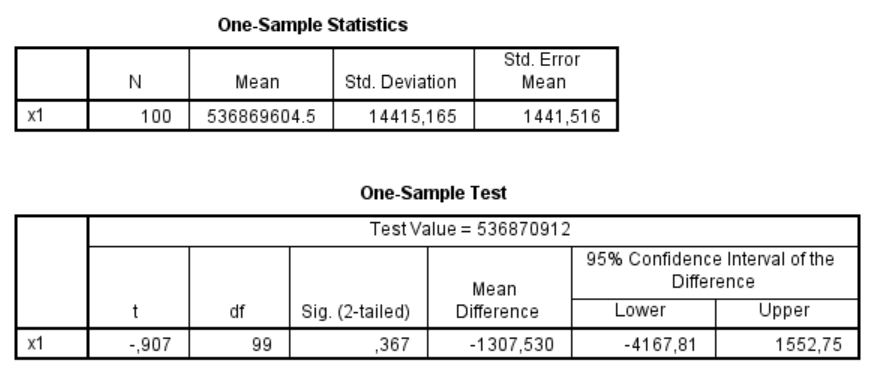
\includegraphics[width=1.0\textwidth]{img/question1/question1_x1_T.PNG}
	\captionsetup{width=1.0\textwidth}
	\centering 
\end{figure}

\paragraph{Conclusion}\mbox{}\\
Because the p-value 0.367 is bigger than 0.05 we conclude there is no significant evidence against our null hypothesis and accept our claim that x1's mean is equal to 536 870 912 Hz.


\subsubsection{T-test Dataset x2}
After executing the T-test on dataset x2 of the crystal oscillators, we get the following tables. Our null hypothesis is that there is no significant difference between dataset x2's mean and given the given average.

\begin{figure}[!htb]
	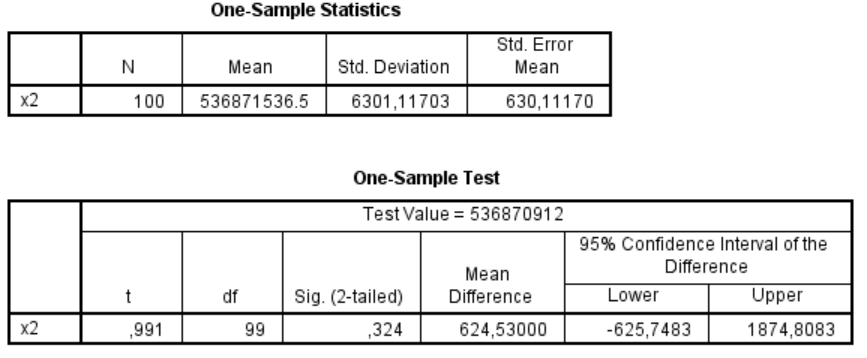
\includegraphics[width=1.0\textwidth]{img/question1/question1_x2_T.PNG}
	\captionsetup{width=1.0\textwidth}
	\centering 
\end{figure}

\paragraph{Conclusion}\mbox{}\\
Because the p-value 0.324 is bigger than 0.05 we conclude there is no significant evidence against our null hypothesis and accept our claim that x2's mean does not differ significantly from 536 870 912 Hz.

\subsection{Crystal Reliability}
Because both dataset means do not differ significantly, are normally distributed and don't differ significantly from the average 536 870 912 Hz, we can trust both crystal types x1 and x2. 

\newpage
\section{Question 2}
We were assigned set 1 for this question, the data represents the number of times visitors bought something or simply left on two variants of a website (site1 and site2). The files whose name ends in a contain the results after 200 visits to each variant.

\begin{figure}[!htb]
	\includegraphics[width=0.7\textwidth]{img/question2/question2_a.PNG}
	\captionsetup{width=0.8\textwidth}
	\centering 
	\caption{The data seems to be a contigency table with the row representing the number of times whether something got bought or not in the two sites. } 
\end{figure}

\subsection{Fisher's Exact Test (set A)}
Because our site data clearly represents a contingency table, we could opt to use either Fisher's Exact Test or Pearson's Chi-Squared Test. However, Fisher's test is more appropriate for small sample size and because the size of our test data (400 site visitors) is fairly low, we opt for Pearson Chi-Squared Test.

\paragraph{Null \& Alternative Hypothesis}\mbox{}\\
For this experiment, our null hypothesis is that there is no significant difference in buying behavior of the two sites. The alternative would be that there is significant difference between the two.

\paragraph{Conclusion}\mbox{}\\
For both the one-sided and two-sided variant of Fisher's Exact Test, we get p-value of 1,000 and 0,500 respectively. This means that we accept the null hypothesis that there is no significant buying behavior between the two sites.

\newpage
\begin{figure}[!htb]
	\includegraphics[width=1.0\textwidth]{img/question2/Question2_Chi.PNG}
	\captionsetup{width=1.0\textwidth}
	\centering 
	%\caption{} 
\end{figure}

\subsection{Chi-Squared Test (set B)}
For set B, we have data of about 500 site visitors. Because we have a bigger sample size than for set B, we now opt to use the non-parametric chi-squared test.

\begin{figure}[!htb]
	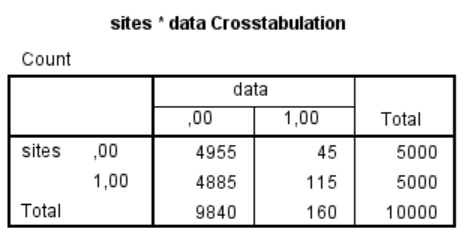
\includegraphics[width=0.7\textwidth]{img/question2/Question2_b.PNG}
	\captionsetup{width=0.8\textwidth}
	\centering 
	\caption{0,00 represents the times a site got visited and nothing got bought. 1,00 is the value for when a site got visited and something got bought.  } 
\end{figure}

\paragraph{Null \& Alternative Hypothesis}\mbox{}\\
Our null hypothesis is that there is no significant difference in buying behavior of the two sites (just a previous test).

\paragraph{Conclusion}\mbox{}\\
We can see that our significance level (p-value) when performing the Pearson Chi-Square test is equal to 0,000 hence less than 0.05. This is why we reject the null hypothesis that the buying behaviour of both sites is equal and we accept the alternate hypothesis that they are different.

\begin{figure}[!htb]
	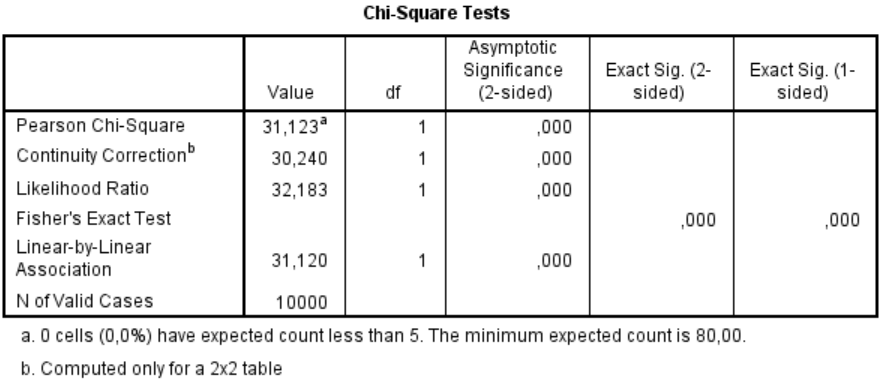
\includegraphics[width=1.0\textwidth]{img/question2/Question2_b_chi.PNG}
	\captionsetup{width=1.0\textwidth}
	\centering 
	%\caption{0,00 represents the times a site got visited and nothing got bought. 1,00 is the value for when a site got visited and something got bought.  } 
\end{figure}

\subsection{Importance of Sample Size}
Sample size is directly related to a statistic's margin of error, or how accurate a statistic can be calculated to be. The bigger the sample size, the less chance there is to wrongfully accept the null hypothesis. 

\section{Question 3}
We are using set number 4 for the fourth question. It deals with the grade difference of a group of students that followed remedial lectures and a control group who did not.

\subsection{Welch's T-Test}
If the variances between the datasets would not differ significantly, we could have opted for a normal independent t-test. Because Levene's test for the equality of variances has a p-value of less than 0.05 (being 0.014), we conclude that both samples their variances differ significantly. Welch's test is a better alternative being robust for independent samples with different variances.

\begin{figure}[!htb]
	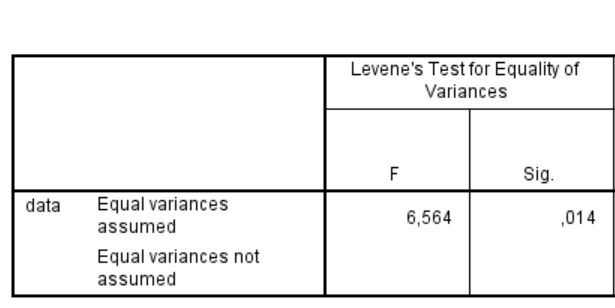
\includegraphics[width=0.8\textwidth]{img/question3/Levene.PNG}
	\captionsetup{width=1.0\textwidth}
	\centering 
\end{figure}

\subsubsection{Null \& Alternative Hypothesis}%\mbox{}\\
Our null hypothesis here is that --for both groups-- the difference in study performance do not differ significantly from one another. If our p-value is smaller than 0.05, we would reject the null hypothesis and accept the alternative hypothesis: the difference is significant.

\begin{figure}[!htb]
	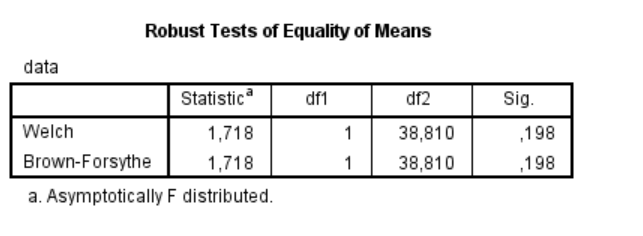
\includegraphics[width=0.9\textwidth]{img/question3/Welch.PNG}
	\captionsetup{width=1.0\textwidth}
	\centering 
\end{figure}

\subsubsection{Conclusion}
Because Welch's test has a p-value of 0.198 (greater than 0.05), we accept the null hypothesis that the means of both dataset are equal. 

\subsection{Statistical Power}
When it comes to hypothesis testing, we can make type I and type II errors. Type I errors occur when we would reject the null hypothesis when it is in fact true, type II errors occur when we would accept the null hypothesis when it is false.
The power of a test is the probability of rejecting the null hypothesis, given it is false. It depends on several factors including the choice of Alpha and the sample size.

\begin{figure}[!htb]
	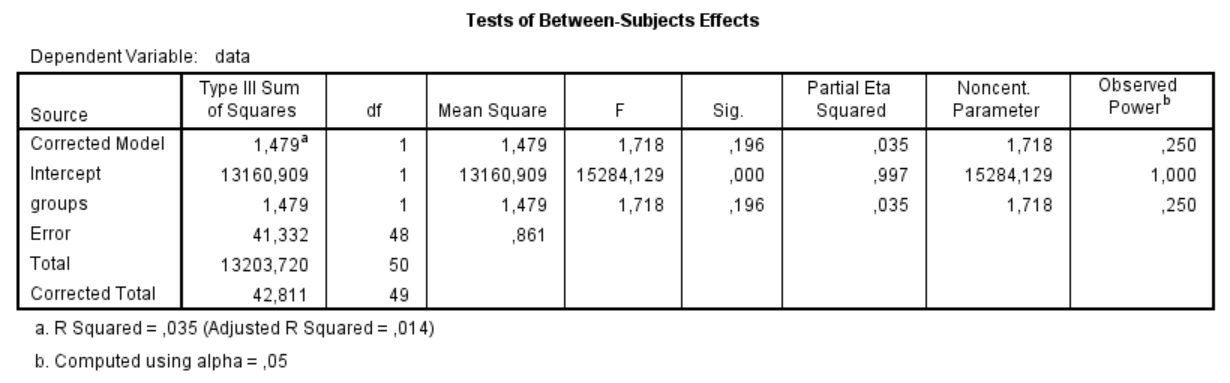
\includegraphics[width=1.0\textwidth]{img/question3/Power.PNG}
	\captionsetup{width=1.0\textwidth}
	\centering 
\end{figure}

\paragraph{Discussion}\mbox{}\\
Our total sample size for this experiment is of 50. With with a p-value of 0.196 and an effect size of 0.035, we can say that there is a 25 \% chance that the detected difference in the test is really there. Hence, the probability of making a type II error would be 75 \%.
\newline 
Having a 75 \% change of accepting the null hypothesis when it is false makes the experiment very unreliable. We must enlarge the sample size to get more reliable results.

\subsection{Power of 0.8}
As to increase our statistical power --hence the chance of distinguishing an actual event of one of change-- we have to change its sample size.

\section{Question 4}
We are using set number 3 for the fourth question as the data of the performance of two algorithms for deep learning. We have to perform regression analysis as to estimate relationships between a dependent variable --hence whether an algorithm was successful in performing a task-- and an independent variable: the number of parameters given to an algorithm.

\subsection{Binary Logistic Regression}
Logistic regression was performed to ascertain the effects of the number of parameters on whether or not the algorithms would solve the tasks. 

\begin{figure}[!htb]
	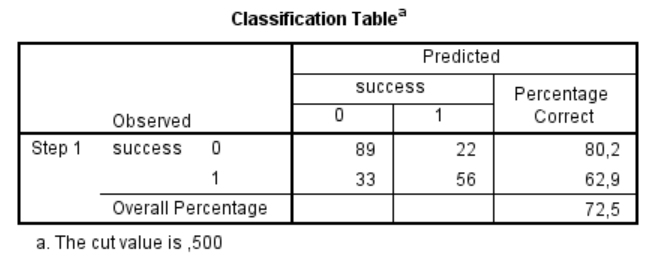
\includegraphics[width=0.8\textwidth]{img/question4/question4_classification.PNG}
	\captionsetup{width=0.8\textwidth}
	\centering 
	\caption{Our model has shown to correctly classify 71.0 \% of cases making it fairly reliable. }
\end{figure}\mbox{}\\

\newpage
\paragraph{Conclusion}\mbox{}\\
In our regression, the first algorithm is encoded as '0' and the second as '1' where we compare the first algorithm with the second algorithm. Underlying variables table in the equation shows that the parameters variable (p = 0,000) adds significantly to our prediction. It is also revealed that the second algorithm fairs 1.069 times better than the second algorithm.

\begin{figure}[!htb]
	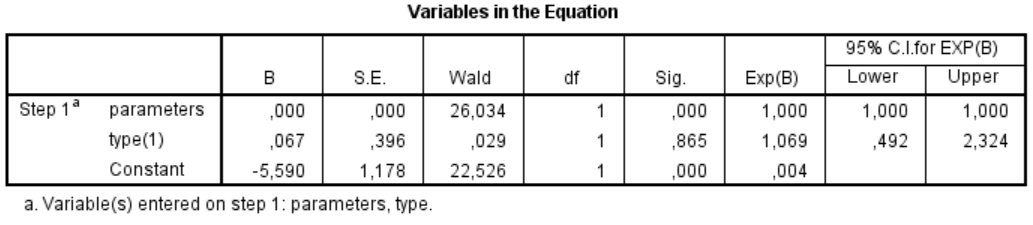
\includegraphics[width=1.0\textwidth]{img/question4/question4_variables.PNG}
	\captionsetup{width=1.0\textwidth}
	\centering 
	%\caption{Our model has shown to correctly classify 71.0 \% of cases making it fairly reliable. }
\end{figure}

\subsection{Succeeding Chance}



\end{document}